\documentclass{article}
\usepackage[utf8]{inputenc}
\usepackage[brazil]{babel}
\usepackage{setspace}
\usepackage{mathtools}
\usepackage{pgfplots}
\usepackage{listings}
\usepackage{xcolor}
\usepackage{natbib}
\usepackage{graphicx}

\DeclarePairedDelimiter\ceil{\lceil}{\rceil}
\DeclarePairedDelimiter\floor{\lfloor}{\rfloor}

\definecolor{codegreen}{rgb}{0,0.6,0}
\definecolor{codegray}{rgb}{0.5,0.5,0.5}
\definecolor{codepurple}{rgb}{0.58,0,0.82}
\definecolor{backcolour}{rgb}{0.95,0.95,0.92}

\lstdefinestyle{codigo}{
    numberstyle=\tiny,
    basicstyle=\ttfamily\footnotesize,
    breakatwhitespace=false,         
    breaklines=true,                 
    captionpos=b,                    
    keepspaces=true,                 
    numbers=left,                    
    numbersep=5pt,                  
    showspaces=false,                
    showstringspaces=false,
    showtabs=false,                  
    tabsize=2
}

\lstset{style=codigo}

\setstretch{1.5}
\pgfplotsset{width=10cm,compat=1.9}

\pagenumbering{gobble}
\clearpage
\thispagestyle{empty}

\title{Lista 2 de Arquitetura de Computadores II}
\author{Gustavo Lopes Rodrigues}
\date{12 de Junho de 2020}



\begin{document}

\maketitle

\section{Parte 1}
\subsection{Programa1}
\lstinputlisting{Lista2/Parte1/Programa1.asm}
\newpage

\subsection{Programa2}
\lstinputlisting{Lista2/Parte1/Programa2.asm}
\newpage

\subsection{Programa3}
\lstinputlisting{Lista2/Parte1/Programa3.asm}
\newpage

\subsection{Programa4}
\lstinputlisting{Lista2/Parte1/Programa4.asm}
\newpage

\subsection{Programa5}
\lstinputlisting{Lista2/Parte1/Programa5.asm}
\newpage

\subsection{Programa6}
\lstinputlisting{Lista2/Parte1/Programa6.asm}
\newpage

\subsection{Programa7}
\lstinputlisting{Lista2/Parte1/Programa7.asm}
\newpage

\subsection{Programa8}
\lstinputlisting{Lista2/Parte1/Programa8.asm}
\newpage

\subsection{Programa9}
\lstinputlisting{Lista2/Parte1/Programa9.asm}
\newpage

\subsection{Programa10}
\lstinputlisting{Lista2/Parte1/Programa10.asm}
\newpage

\subsection{Programa11}
\lstinputlisting{Lista2/Parte1/Programa11.asm}
\newpage

\section{Parte 2}
\subsection{Programa1}
\lstinputlisting{Lista2/Parte2/Programa1.asm}
\newpage

\subsection{Programa2}
\lstinputlisting{Lista2/Parte2/Programa2.asm}
\newpage

\subsection{Programa3}
\lstinputlisting{Lista2/Parte2/Programa3.asm}
\newpage

\subsection{Programa4}
\lstinputlisting{Lista2/Parte2/Programa4.asm}
\newpage

\subsection{Programa5}
\lstinputlisting{Lista2/Parte2/Programa5.asm}
\newpage

\subsection{Programa6}
\lstinputlisting{Lista2/Parte2/Programa6.asm}
\newpage

\subsection{Programa7}
\lstinputlisting{Lista2/Parte2/Programa7.asm}
\newpage

\subsection{Programa8}
\lstinputlisting{Lista2/Parte2/Programa8.asm}
\newpage

\subsection{Programa9}
\lstinputlisting{Lista2/Parte2/Programa9.asm}
\newpage

\subsection{Programa10}
\lstinputlisting{Lista2/Parte2/Programa10.asm}
\newpage

\subsection{Programa11}
\lstinputlisting{Lista2/Parte2/Programa11.asm}
\newpage

\subsection{Programa12}
\lstinputlisting{Lista2/Parte2/Programa12.asm}
\newpage

\subsection{Programa13}
\lstinputlisting{Lista2/Parte2/Programa13.asm}
\newpage

\subsection{Programa14}
\lstinputlisting{Lista2/Parte2/Programa14.asm}
\newpage

\subsection{Programa15}
\lstinputlisting{Lista2/Parte2/Programa15.asm}
\newpage

\subsection{Programa16}
\lstinputlisting{Lista2/Parte2/Programa16.asm}
\newpage

\subsection{Programa17}
\lstinputlisting{Lista2/Parte2/Programa17.asm}
\newpage

\subsection{Programa18}
\lstinputlisting{Lista2/Parte2/Programa18.asm}
\newpage

\subsection{Programa19}
\lstinputlisting{Lista2/Parte2/Programa19.asm}
\newpage

\subsection{Programa20}
\lstinputlisting{Lista2/Parte2/Programa20.asm}
\newpage

\subsection{Programa21}
\lstinputlisting{Lista2/Parte2/Programa21.asm}
\newpage

\subsection{Programa22}
\lstinputlisting{Lista2/Parte2/Programa22.asm}
\newpage

\subsection{Programa23}
\lstinputlisting{Lista2/Parte2/Programa23.asm}
\newpage

\subsection{Programa24}
\lstinputlisting{Lista2/Parte2/Programa24.asm}
\newpage

\subsection{Programa25}
\lstinputlisting{Lista2/Parte2/Programa25.asm}
\newpage

\section{Parte 3}
\subsection{Programa1}
\lstinputlisting{Lista2/Parte3/Programa1.asm}
\newpage

\subsection{Programa2}
\lstinputlisting{Lista2/Parte3/Programa2.asm}
\newpage

\subsection{Programa3}
\lstinputlisting{Lista2/Parte3/Programa3.asm}
\newpage

\subsection{Programa4}
\lstinputlisting{Lista2/Parte3/Programa4.asm}
\newpage

\subsubsection{Programa4 Adicionando nops}
\lstinputlisting{Lista2/Parte3/Programa4_1.asm}
\newpage

Fazendos os calculos(Programa4):
\newline
Instruções da ALU:    3 | 78\%| 2,34
\newline
Instruções de desvio: 4 | 11\%| 0,44
\newline
Instruções de MEM:    5 | 11\%| 0,55
\newline
\begin{equation}
CPI Medio = \frac{3*78\%+4*11\%+5*11\%}{12} = 0,2775
\end{equation}
\newline
Tempo de execução = 0,2775*12*10us = 0,00000333ms
\newline
\newline
(Programa4 com nops):
\newline
Instruções da ALU:    3 | 72\%| 2,16
\newline
Instruções de desvio: 4 | 14\%| 0,56
\newline
Instruções de MEM:    5 | 14\%| 0,7
\newline
\begin{equation}
CPI Medio = \frac{3*72\%+4*14\%+5*14\%}{12} = 0,285
\end{equation}
\newline
Tempo de execução = 0,285*12*10us = 0,00000342ms
\newline
Speedup = 0,00000333ms / 0,00000342ms = 1,027 = 2,7\%
\newpage

\subsection{Programa5}
\lstinputlisting{Lista2/Parte3/Programa5.asm}
\newpage

\subsubsection{Programa5 Adicionando nops}
\lstinputlisting{Lista2/Parte3/Programa5_1.asm}
\newpage
Fazendos os calculos(Programa4):
\newline
Instruções da ALU:    3 | 50\%| 1,5
\newline
Instruções de desvio: 4 | 17\%| 0,68
\newline
Instruções de MEM:    5 | 33\%| 1,65
\newline
\begin{equation}
CPI Medio = \frac{3*50\%+4*17\%+5*33\%}{12} = 0,31916666666
\end{equation}
\newline
Tempo de execução = 0,31916666666*12*10us = 0,0000038299ms
\newline
\newline
(Programa4 com nops):
\newline
Instruções da ALU:    3 | 63\%| 1,89
\newline
Instruções de desvio: 4 | 12\%| 0,48
\newline
Instruções de MEM:    5 | 25\%| 1,25
\newline
\begin{equation}
CPI Medio = \frac{3*63\%+4*12\%+5*25\%}{12} = 0,30166666666
\end{equation}
\newline
Tempo de execução = 0,30166666666*12*10us = 0,00000361999ms
\newline
Speedup = 0,0000038299ms / 0,00000361999ms = 1,057 = 5,7\%
\newpage
\subsection{Programa6}
\lstinputlisting{Lista2/Parte3/Programa6.asm}
\newpage

\subsection{Programa7}
\lstinputlisting{Lista2/Parte3/Programa7.asm}
\newpage

\section{Parte 4}
\subsection{Questão 1}
\lstinputlisting{Lista2/Parte4/Questao1.asm}
\newpage

\subsection{Questão 2}
\centering
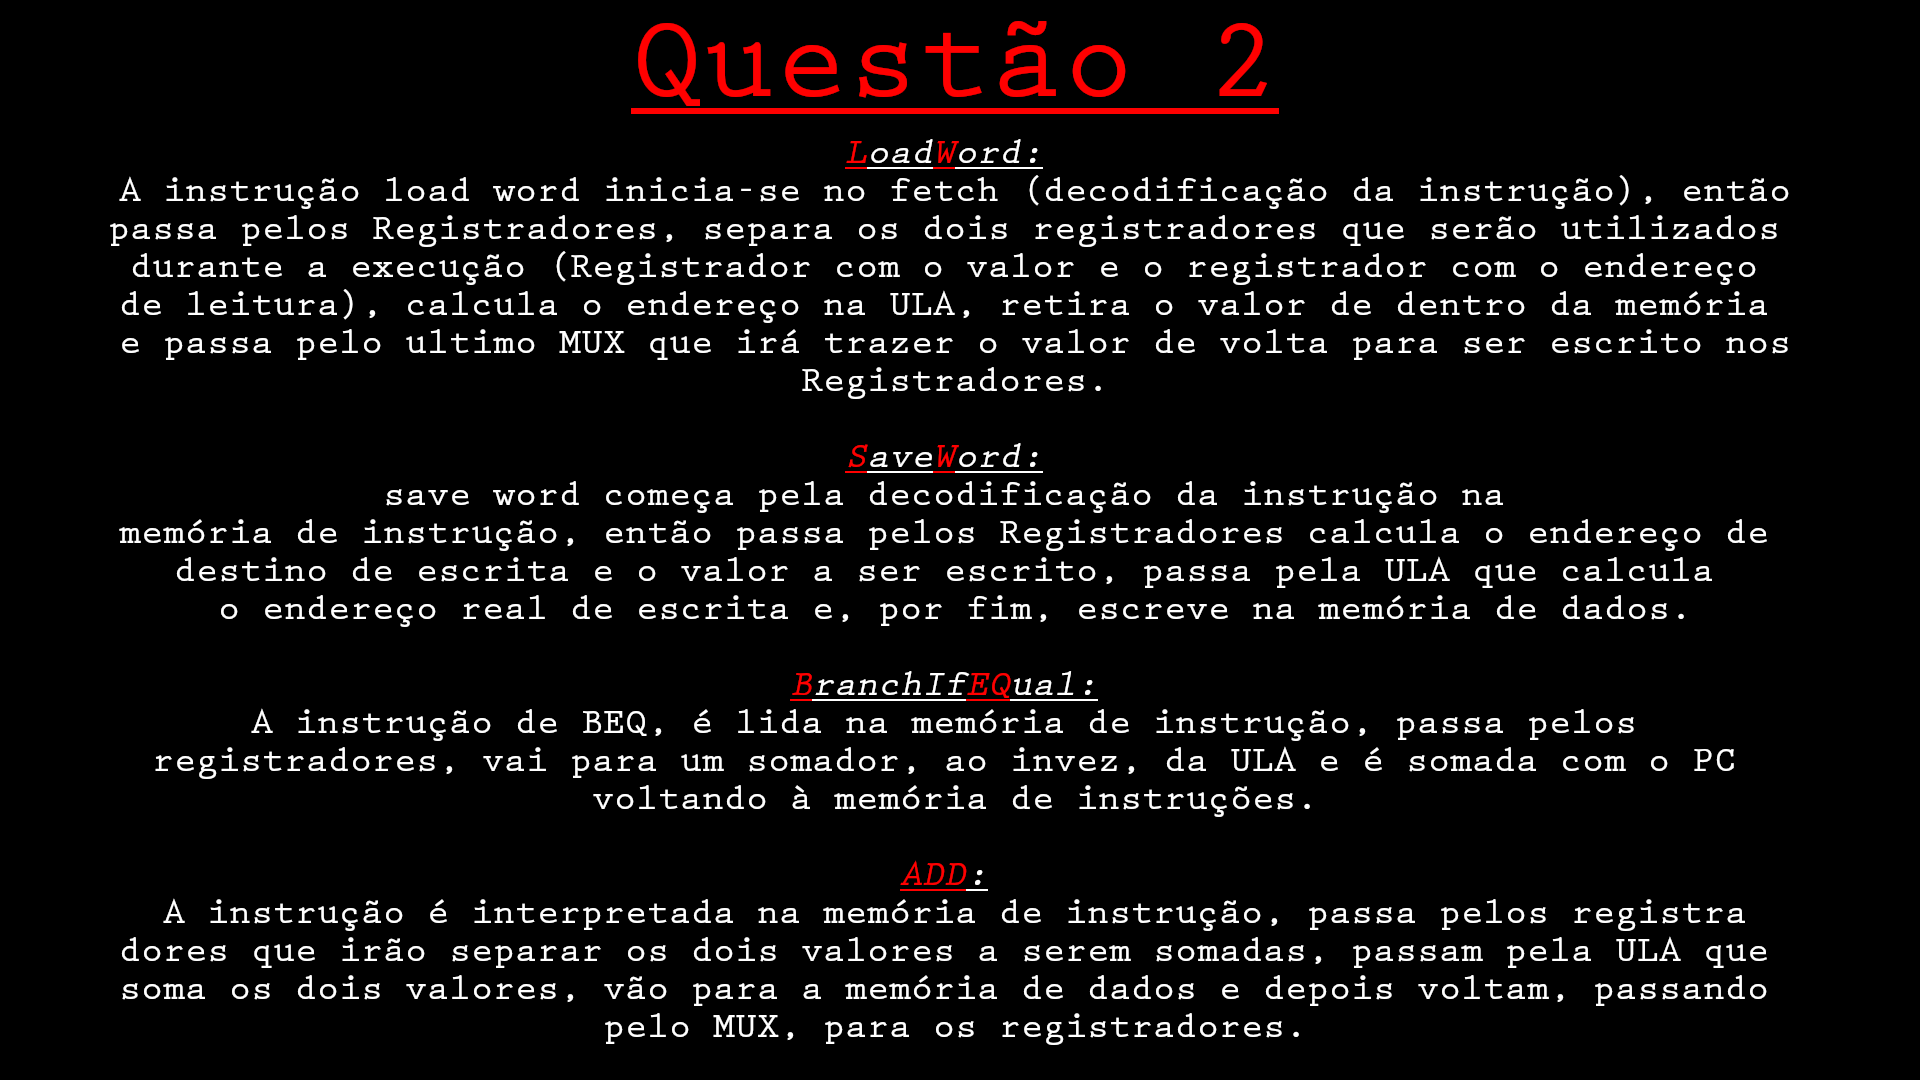
\includegraphics{Lista2/Parte4/Questao2.png}
\newpage

\subsection{Questão 3}
\centering
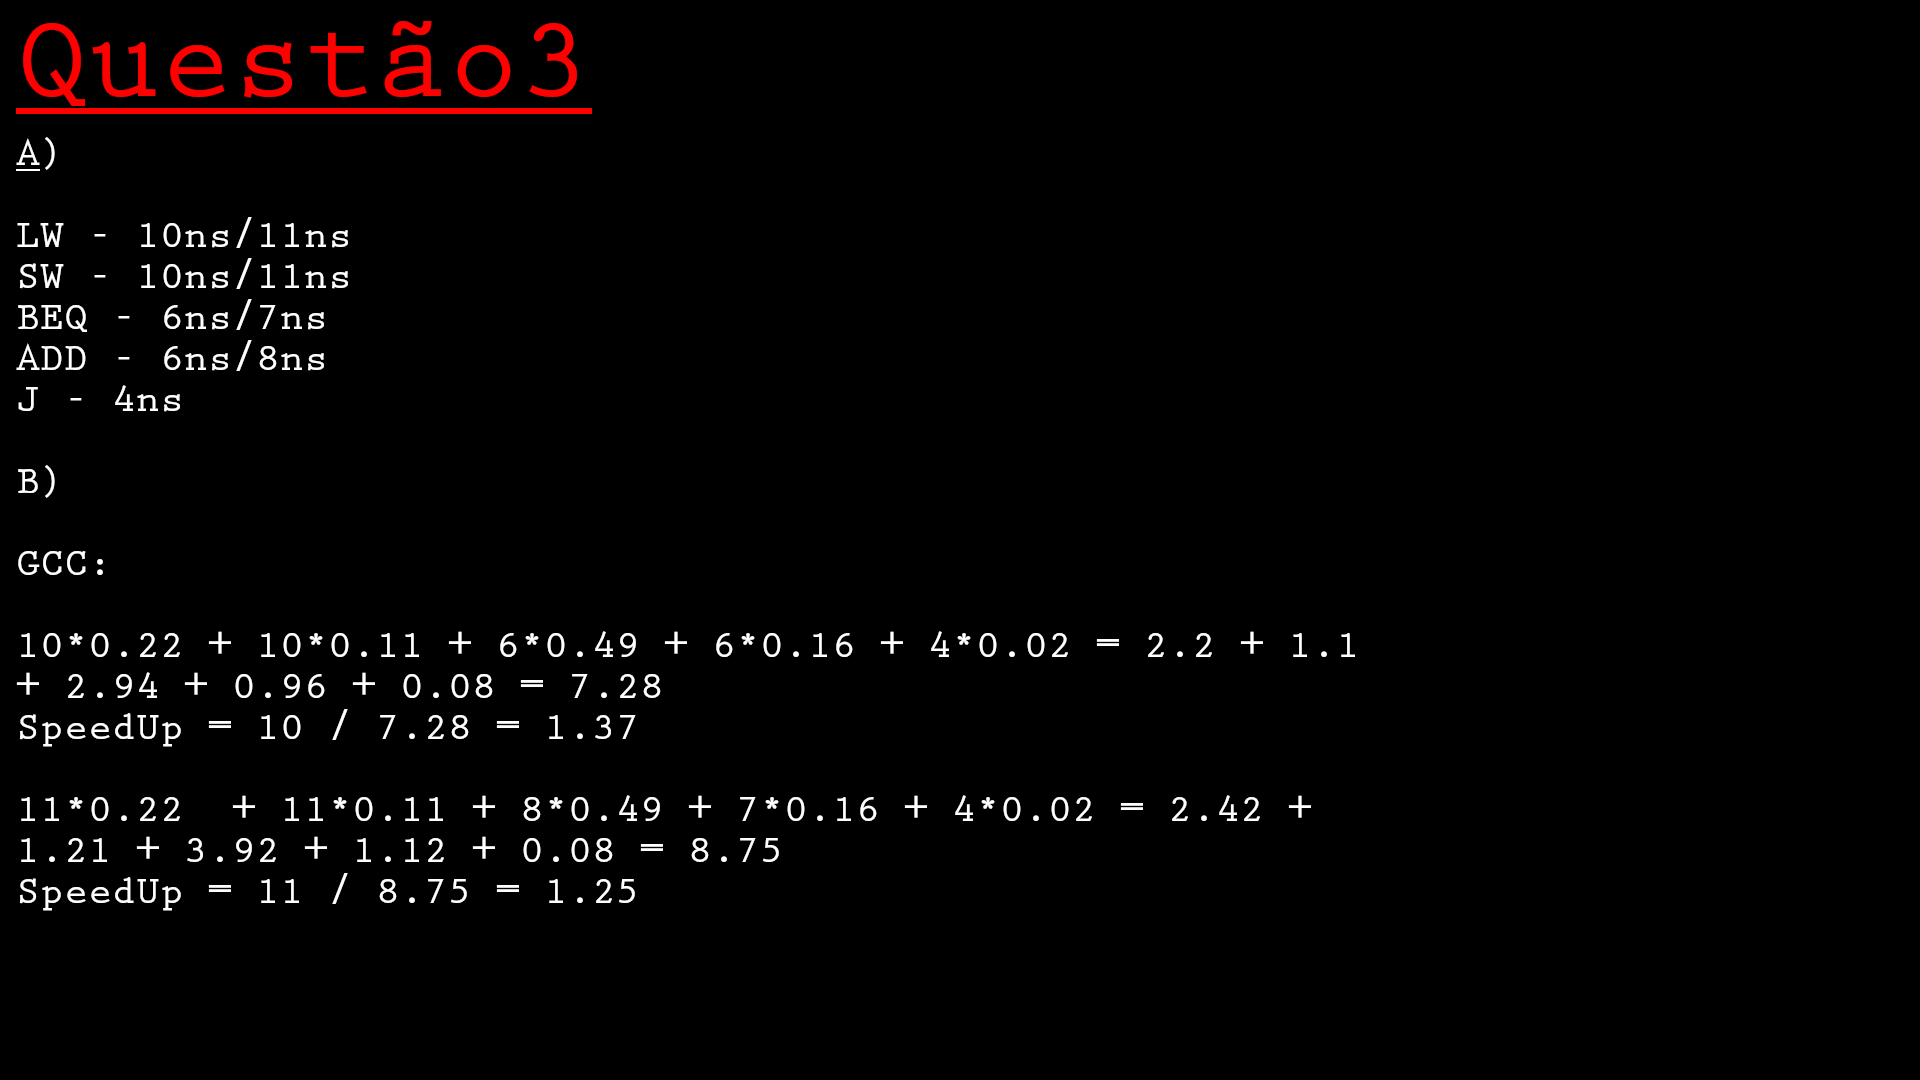
\includegraphics{Lista2/Parte4/Questao3.png}
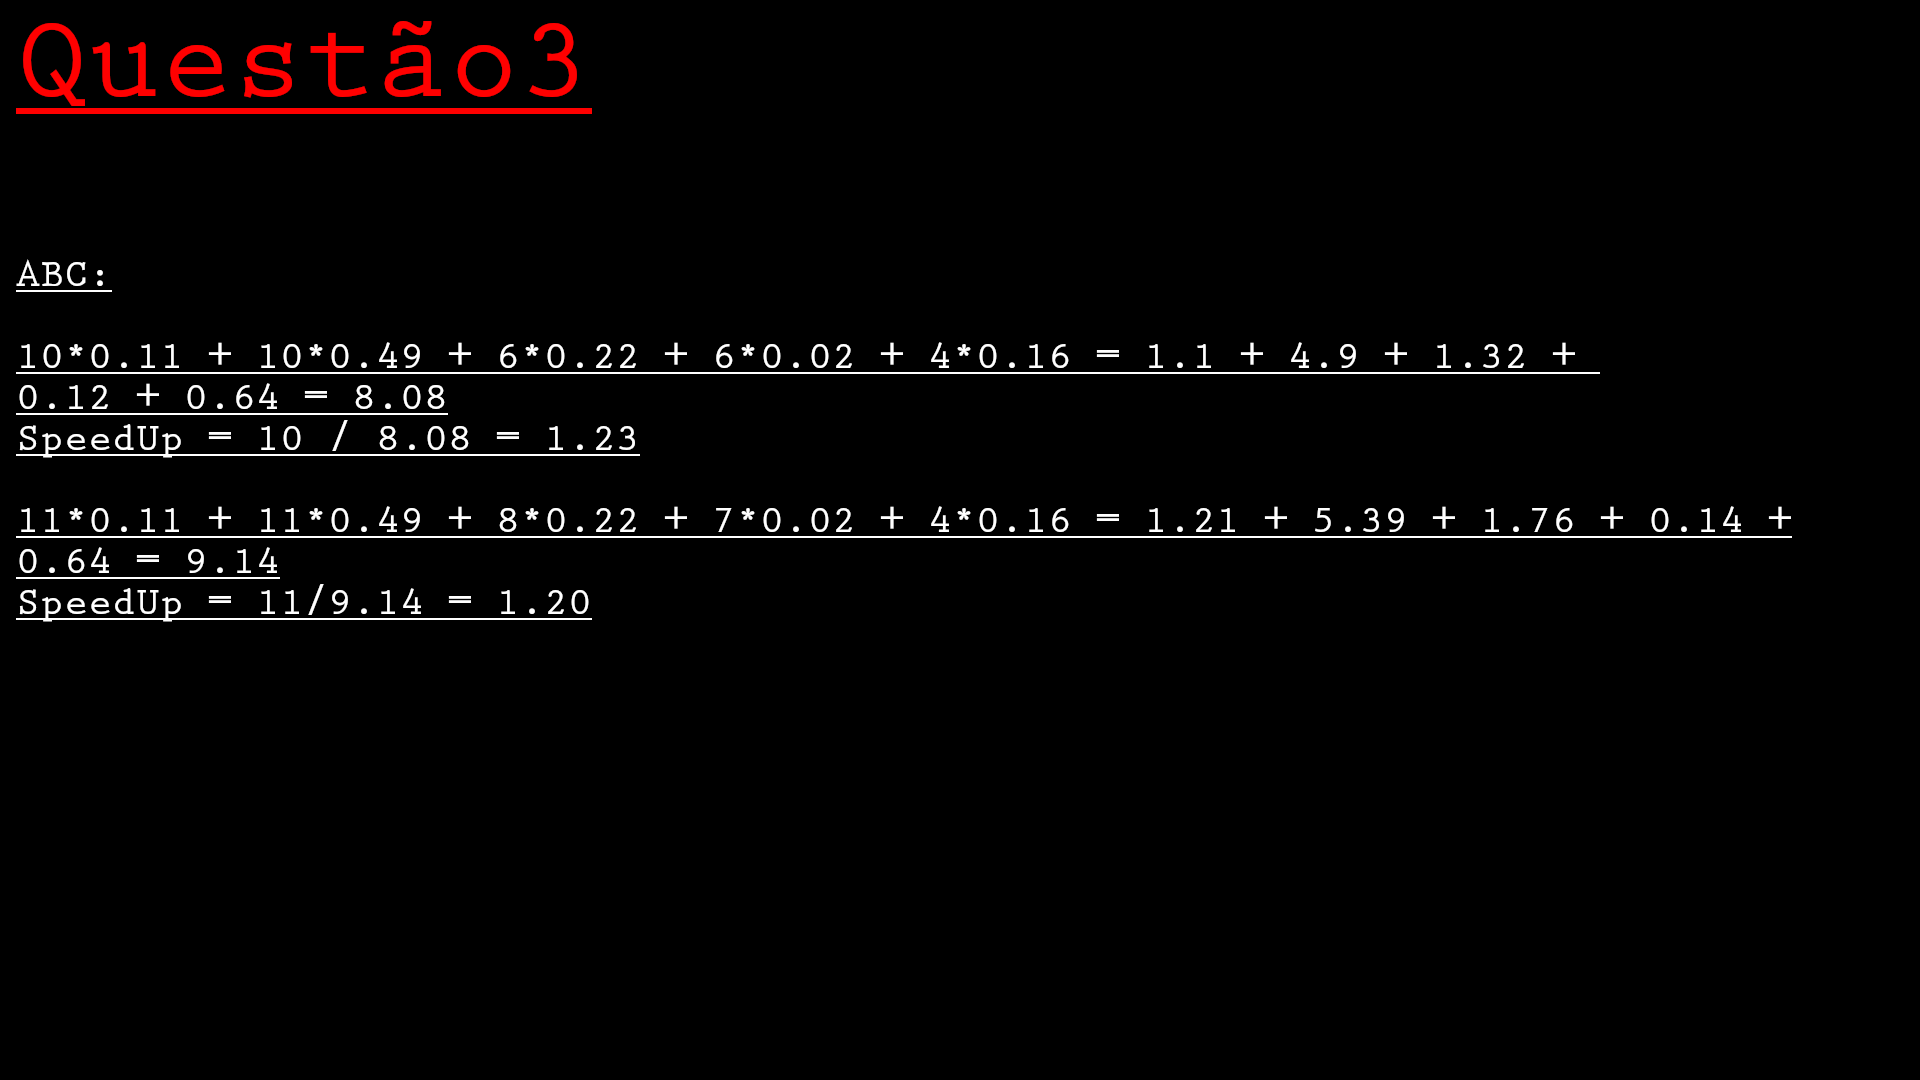
\includegraphics{Lista2/Parte4/Questao3_1.png}
\newpage

\subsection{Questão 4}
\centering
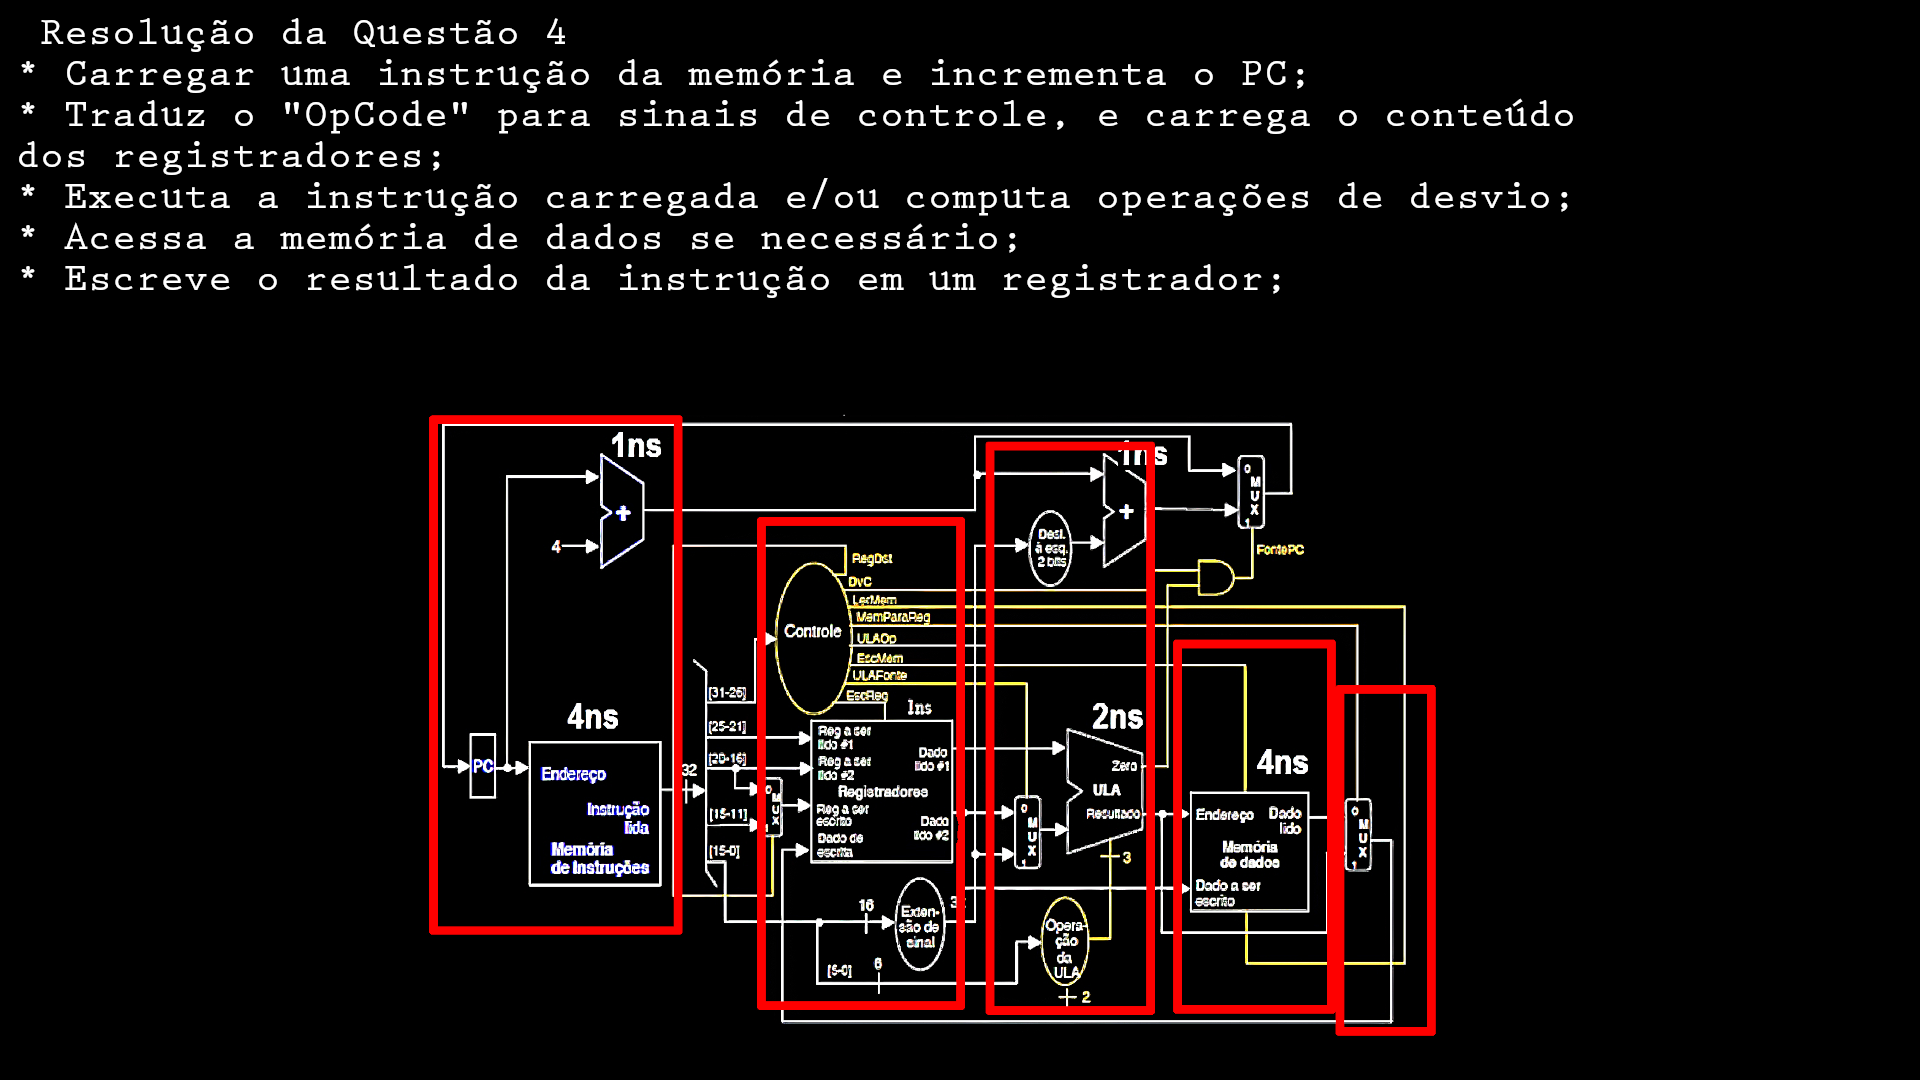
\includegraphics{Lista2/Parte4/Questao4.png}
\newpage

\end{document}